 % gjilguid2e.tex
% V2.0 released 1998 December 18
% V2.1 released 2003 October 7 -- Gregor Hutton, updated the web address for the style files.

%\documentclass{gji}
%\documentclass[extra,mreferee]{gji}
\documentclass[mreferee]{gji}
\usepackage{gji_extra}
\usepackage{timet}
%\usepackage{units, amstext, amsmath, amssymb, stfloats, graphics, setspace, dcolumn}
\usepackage{units, amstext, amsmath, amssymb} % There is a problem with some of the above packages
\usepackage{graphicx}
\usepackage{caption}
%\usepackage{subcaption} % There is a problem with this package
\usepackage{subfig}

\title[Differential operators in geodetic coordinates] % short title
  {Differential operators in geodetic coordinates applied to potential-field modelling} % main title
\author[K. A. T. Hallam, V. C. Oliveira Jr.] % first page
  {K. A. T. Hallam$^1$, V. C. Oliveira Jr.$^1$ %
  \\
  $^1$ Department of Geophysics, Observat\'{o}rio Nacional, Rio de Janeiro
  , Brazil
  }
%\date{Received 1998 December 18; in original form 1998 November 22}
\pagerange{\pageref{firstpage}--\pageref{lastpage}}
%\volume{200}
\pubyear{2017}

\def\LaTeX{L\kern-.36em\raise.3ex\hbox{{\small A}}\kern-.15em
    T\kern-.1667em\lower.7ex\hbox{E}\kern-.125emX}
\def\LATeX{L\kern-.36em\raise.3ex\hbox{{\Large A}}\kern-.15em
    T\kern-.1667em\lower.7ex\hbox{E}\kern-.125emX}
% Authors with AMS fonts and mssymb.tex can comment out the following
% line to get the correct symbol for Geophysical Journal International.
\let\leqslant=\leq

%\newtheorem{theorem}{Theorem}[section]

\begin{document}

\label{firstpage}

\maketitle


\begin{summary}


TEXT TEXT TEXT


\end{summary}


\begin{keywords}
%\LaTeXe\ -- class files: \verb"gji.cls"\ -- sample text -- user guide.
Numerical modelling, Gravity anomalies and Earth structure, Magnetic anomalies: modelling and interpretation
\end{keywords}


\section{Introduction} \label{sec.intro}


Several methods have been developed to
compute the gravitational and magnetic fields produced by
geological structures in Cartesian (CITAR PAPERS CLASSICOS)
and spherical coordinates (CITAR PAPERS CLASSICOS).

The spherical approach is more appropriated than the Cartesian approach
for modelling large-scale structures which require taking the Earth's
curvature into account.

The spherical approach, however, neglects the Earth's ellipticity.

\citet{roussel2015} is the only work presenting a potential-field modelling
that takes the Earth's ellipticity into consideration.
Their method is formulated in ellipsoidal coordinates and
relies on the numerical solution of volume integrals by applying
Gauss-Legendre quadrature.

The gravitational and magnetic fields computed by these methods cannot
be directly compared to geophysical observations because the position of
the last ones are commonly described in geodetic coordinates  
\citep[e.g.,][]{hotine1969, heiskanen-moritz1967, krakiwsky1971, soler1976,
vanicek1987, rapp1991, seeber2003, hofmann-wellenhof-moritz2005, torge2012}.

Consequently, coordinate transformations are required.

Up to now, the geoscientific community lacks of methods for computing
the gravitational and magnetic fields produced by geological bodies
in geodetic coordinates.

We present the differential operators gradient, divergent,
Laplacian and curl in terms of the scale factors and the
normal basis associated to the GCS.

We applied the differential operators presented here to
define the expressions of the gravitational and magnetic fields
produced by spheres.

Such expressions are can be used, for example, for producing regional
magnetic anomaly maps \citep[e.g.,][]{vonfrese-etal1981, mayhew1982, dyment1998},
characterizing the regional gravity field \citep[e.g.,][]{needham1970, balmino1972,
barthelmes1991, barthelmes1991b, lehmann1993, antunes2003, guspi2004, lin2014} or
approximating the gravitational and magnetic fields produced by geological
structures with arbitrary shapes.

%Finally, we also provide a set of routines developed in Python language...


\section{Geodetic curvilinear coordinates}


\subsection{Relationship between Cartesian and Geodetic coordinates}


Consider a terrestrial geocentric system of Cartesian coordinates
having the $z$-axis coincident with the mean rotational axis,
the $x$-axis pointing to the Greenwich meridian and the $y$-axis
directed so as to obtain a right-handed system
(Fig. \ref{fig:cartesian-geodetic-systems}).
Coordinate systems similar to this one may be found in the literature as
Conventional Terrestrial Reference Coordinate System \citep[e.g.,][]{soler1988}, 
International Terrestrial Reference System \citep[e.g.,][]{seeber2003, torge2012} 
or Earth-centered Earth-fixed system \citep[e.g.,][]{bouman2013}, for example.
Here, we opted for simply using the term Geocentric Cartesian System
(GCS).
Let us also consider a terrestrial geocentric system of geodetic coordinates
$h$ (geometric height), $\varphi$ (geodetic latitude), and 
$\lambda$ (longitude) defined with respect to a reference ellipsoid
of revolution having major semi-axis $a$ and minor semi-axis $b$.
For convenience, we call this system Geocentric Geodetic System
(GGS).

The geodetic coordinates $h$, $\varphi$, and $\lambda$ can be transformed
into the Cartesian coordinates $x$, $y$, and $z$ as follows
\citep{heiskanen-moritz1967}:
\begin{equation} \label{eq:geodetic-2-cartesian}
\begin{split}
x &= \left( N + h \right) \, \cos\varphi \, \cos\lambda \\ 
y &= \left( N + h \right) \, \cos\varphi \, \sin\lambda \\
z &= \left[ N \left( 1 - e^{2} \right) + h \right] \, \sin\varphi
\end{split} \: ,
\end{equation}
where $e = \sqrt{a^{2} - b^{2}}/a$ is the first eccentricity and
$N$ is the prime vertical radius of curvature given by
\begin{equation} \label{eq:N-prime-radius}
N = \frac{a}{\left( 1 - e^{2} \sin^{2}\varphi \right)^{\frac{1}{2}}} \: .
\end{equation}
Additionally, let us define the meridian radius of curvature $M$ as
follows:
\begin{equation} \label{eq:M-meridian-radius}
M = \frac{a \left( 1 - e^{2} \right)}{\left( 1 - e^{2} \sin^{2}\varphi \right)^{\frac{3}{2}}} \: .
\end{equation}
It can be easily verified that the prime vertical radius of curvature $N$
(eq. \ref{eq:N-prime-radius}), the meridian radius of curvature $M$
(eq. \ref{eq:M-meridian-radius}) and their first derivatives with respect to
$\varphi$ satisfy the following relationships:
\begin{equation} \label{eq:relation-betwen-N-M}
M = \frac{1 - e^{2}}{1 - e^{2} \sin^{2}\varphi} N
\end{equation}
and
\begin{equation} \label{eq:N-derivative}
\frac{\partial N}{\partial \varphi} = \frac{e^{2} \, \sin \varphi \, \cos \varphi}{1 - e^{2} \sin^{2}\varphi} N \: .
\end{equation}


\subsection{Scale factors and local basis of the GGS}


Having defined the relations between the Cartesian and geodetic coordinates,
we will now apply some well-established concepts of generic curvilinear
coordinates. An in-depth presentation of these concepts may be found at
\citet{kellogg1929}, \citet{hotine1969}, \citet{arfken2001}, or \citet{sttraton2007},
for example. We shall confine ourselves to
the particular case of geodetic curvilinear coordinates.

Let us first make use of the Pythagorean theorem to define the
squared magnitude of the infinitesimal displacement between two
neighbouring points in the GCS system is given by
\begin{equation} \label{eq:ds2-cartesian}
ds^{2} = dx^{2} + dy^{2} + dz^{2} \: ,
\end{equation}
where the differentials $dx$, $dy$, and $dz$ are obtained from
eqs \ref{eq:geodetic-2-cartesian} as follows:
\begin{equation} \label{eq:dalpha}
d\alpha = \frac{\partial \alpha}{\partial h} \, dh +
\frac{\partial \alpha}{\partial \varphi} \, d\varphi +
\frac{\partial \alpha}{\partial \lambda} \, d\lambda
\: , \quad \alpha = x, y, z \: ,
\end{equation}
and the partial derivatives $\frac{\partial \alpha}{\partial \beta}$,
$\alpha = x, y, z$, $\beta = h, \varphi, \lambda$, are given by \citep{soler1976}:
\begin{equation} \label{eq:dalpha-dbeta}
\begin{array}{ccc}
\frac{\partial x}{\partial h} = \cos\varphi \, \cos\lambda &
\frac{\partial x}{\partial \varphi} = -\left( M + h \right) \, \sin\varphi \, \cos\lambda &
\frac{\partial x}{\partial \lambda} = -\left( N + h \right) \, \cos\varphi \, \sin\lambda \\
\frac{\partial y}{\partial h} = \cos\varphi \, \sin\lambda &
\frac{\partial y}{\partial \varphi} = -\left( M + h \right) \, \sin\varphi \, \sin\lambda &
\frac{\partial y}{\partial \lambda} = \left( N + h \right) \, \cos\varphi \, \cos\lambda \\
\frac{\partial z}{\partial h} = \sin\varphi &
\frac{\partial z}{\partial \varphi} = \left( M + h \right) \, \cos\varphi &
\frac{\partial z}{\partial \lambda} = 0 \\
\end{array} \: .
\end{equation}
The partial derivatives with respect to $\varphi$ were deduced from
eqs \ref{eq:geodetic-2-cartesian} by using
eqs \ref{eq:relation-betwen-N-M} and \ref{eq:N-derivative}.

From these differentials $d\alpha$ (eqs \ref{eq:dalpha}), we define the
Jacobian matrix
\begin{equation} \label{eq:Jacobian-matrix}
\mathbf{J} = \begin{bmatrix}
\frac{\partial x}{\partial h} & \frac{\partial x}{\partial \varphi} & \frac{\partial x}{\partial \lambda} \\
\frac{\partial y}{\partial h} & \frac{\partial y}{\partial \varphi} & \frac{\partial y}{\partial \lambda} \\
\frac{\partial z}{\partial h} & \frac{\partial z}{\partial \varphi} & \frac{\partial z}{\partial \lambda}
\end{bmatrix} \: .
\end{equation}

By substituting the differentials $d\alpha$ (eqs \ref{eq:dalpha}) into
eq. \ref{eq:ds2-cartesian}, we obtain a general quadratic form
representing the squared distance $ds^{2}$ given by
\begin{equation} \label{eq:ds2}
ds^{2} = g_{11} \, dh^{2} + g_{22} \, d\varphi^{2} + g_{33} \, d\lambda^{2} + 
2 \left( g_{12} \, dh \, d\varphi + g_{13} \, dh \, d\lambda +
g_{23} \, d\varphi \, d\lambda \right) \: ,
\end{equation}
where
\begin{equation} \label{eq:metric-coeffs-gii}
\begin{split}
g_{11} &= \left( \frac{\partial x}{\partial h} \right)^{2}
+ \left( \frac{\partial y}{\partial h} \right)^{2} +
\left( \frac{\partial z}{\partial h} \right)^{2} \\
g_{22} &= \left( \frac{\partial x}{\partial \varphi} \right)^{2}
+ \left( \frac{\partial y}{\partial \varphi} \right)^{2} +
\left( \frac{\partial z}{\partial \varphi} \right)^{2} \\
g_{33} &= \left( \frac{\partial x}{\partial \lambda} \right)^{2}
+ \left( \frac{\partial y}{\partial \lambda} \right)^{2} +
\left( \frac{\partial z}{\partial \lambda} \right)^{2}
\end{split} \quad ,
\end{equation}
and
\begin{equation} \label{eq:metric-coeffs-gij}
\begin{split}
g_{12} &=
\left( \frac{\partial x}{\partial h} \, \frac{\partial x}{\partial \varphi} \right) +
\left( \frac{\partial y}{\partial h} \, \frac{\partial y}{\partial \varphi} \right) +
\left( \frac{\partial z}{\partial h} \, \frac{\partial z}{\partial \varphi} \right) \\
g_{13} &=
\left( \frac{\partial x}{\partial h} \, \frac{\partial x}{\partial \lambda} \right) +
\left( \frac{\partial y}{\partial h} \, \frac{\partial y}{\partial \lambda} \right) +
\left( \frac{\partial z}{\partial h} \, \frac{\partial z}{\partial \lambda} \right) \\
g_{23} &=
\left( \frac{\partial x}{\partial \varphi} \, \frac{\partial x}{\partial \lambda} \right) +
\left( \frac{\partial y}{\partial \varphi} \, \frac{\partial y}{\partial \lambda} \right) +
\left( \frac{\partial z}{\partial \varphi} \, \frac{\partial z}{\partial \lambda} \right)
\end{split} \quad .
\end{equation}
The coefficients defined by eqs \ref{eq:metric-coeffs-gii} and
\ref{eq:metric-coeffs-gij} are commonly called metrical coefficients.
It can be shown that the coefficients $g_{12}$, $g_{13}$, and $g_{23}$
(eqs \ref{eq:metric-coeffs-gij}) are equal to zero, which implies that
the GGS is an orthogonal system.

The squared infinitesimal distance $ds^{2}$ (eq. \ref{eq:ds2})
can be rewritten as follows:
\begin{equation} \label{eq:ds2-orthogonal}
ds^{2} = \left( h_{1} \, dh \right)^{2} + 
\left( h_{2} \, d\varphi \right)^{2} + \left( h_{3} \, d\lambda \right)^{2} \: ,
\end{equation}
where $h_{i}$, $i = 1, 2, 3$, are called scale factors.
These coefficients are defined as the square root of the metrical coefficients
$g_{ii}$ (eqs \ref{eq:metric-coeffs-gii}) as follows:
\begin{equation} \label{eq:scale-factors-hi}
\begin{split}
h_{1} &= 1 \\
h_{2} &= M + h \\
h_{3} &= \left( N + h \right) \cos\varphi
\end{split} \quad ,
\end{equation}
where $N$ and $M$ are defined by eqs \ref{eq:N-prime-radius} and
\ref{eq:M-meridian-radius}, respectively.
Notice that, in eq. \ref{eq:ds2-orthogonal}, the terms
$h_{1} \, dh$, $h_{2} \, d\varphi$, and $h_{3} \, d\lambda$
represent infinitesimal displacement components along the geodetic
coordinates $h$, $\varphi$, and $\lambda$, respectively.
By using the scale factors $h_{1}$, $h_{2}$, and $h_{3}$ (eqs \ref{eq:scale-factors-hi}),
we may define the metric matrix $\mathbf{H}$ \citep{soler1976} as follows:
\begin{equation} \label{eq:H-metric-matrix}
\mathbf{H} = \begin{bmatrix}
h_{1} & & \\
& h_{2} & \\
& & h_{3}
\end{bmatrix} \: .
\end{equation}

It is also necessary to define a set of mutually orthogonal vectors at
a given fixed point.
To do this, let us first define the \textit{position vector} 
$\mathbf{r}$ with elements defined by the Cartesian coordinates
$x$, $y$ and $z$ (eq. \ref{eq:geodetic-2-cartesian}) as follows:
\begin{equation} \label{eq:position-vector}
\mathbf{r} = \begin{bmatrix}
x(h, \varphi, \lambda) \\
y(h, \varphi, \lambda) \\
z(h, \varphi, \lambda)
\end{bmatrix} \: .
\end{equation}
Then, the set of mutually orthogonal vectors can be
given by
\begin{equation} \label{eq:unitary-vectors}
\begin{split}
\mathbf{e}_{1} &= \frac{\partial \mathbf{r}}{\partial h} \\
\mathbf{e}_{2} &= \frac{\partial \mathbf{r}}{\partial \varphi} \\
\mathbf{e}_{3} &= \frac{\partial \mathbf{r}}{\partial \lambda}
\end{split} \: .
\end{equation}
Such vectors are called \textit{unitary vectors} \citep{sttraton2007}.
Notice that the unitary vectors $\mathbf{e}_{1}$, $\mathbf{e}_{2}$, and $\mathbf{e}_{3}$
are defined, respectively, in the direction of the increasing geodetic coordinates
$h$, $\varphi$, and $\lambda$.
Besides, the magnitude of a unitary vector $\mathbf{e}_{i}$ is equal to
the scale factor $h_{i}$, $i = 1, 2, 3$,
which shows that it is not necessarily a unit vector.
By multiplying the unitary vectors $\mathbf{e}_{i}$ (eq. \ref{eq:unitary-vectors})
by the reciprocal of the scale factors $h_{i}$ (eq. \ref{eq:scale-factors-hi})
and using the partial derivatives defines by eqs \ref{eq:dalpha-dbeta},
we obtain a set of three mutually orthogonal unit vectors given by \citep{soler1976}
\begin{equation} \label{eq:unit-vectors}
\begin{split}
\hat{\mathbf{e}}_{1} &= 
\begin{bmatrix}
\cos\varphi \, \cos\lambda \\
\cos\varphi \, \sin\lambda \\
\sin\varphi
\end{bmatrix} \\
\hat{\mathbf{e}}_{2} &= 
\begin{bmatrix}
-\sin\varphi \, \cos\lambda \\
-\sin\varphi \, \sin\lambda \\
\cos\varphi
\end{bmatrix} \\
\hat{\mathbf{e}}_{3} &= 
\begin{bmatrix}
-\sin\lambda \\
\cos\lambda \\
0
\end{bmatrix}
\end{split} \: ,
\end{equation}
where $N$ and $M$ are defined by eqs \ref{eq:N-prime-radius} and
\ref{eq:M-meridian-radius}, respectively.
These vectors form a local orthonormal basis in the space of Cartesian
coordinates.
By using these vectors (eqs \ref{eq:unit-vectors}), we can define the
matrix equation transforming a vector $\mathbf{v}_{C}$, defined at a
point in the GCS, into a vector $\mathbf{v}_{G}$, defined 
at the same point in the GGS, as follows:
\begin{equation} \label{eq:vC-2-vG}
\mathbf{v}_{G} = \mathbf{R}^{\top} \mathbf{v}_{C} \: ,
\end{equation}
where $\mathbf{R}$ is a rotation matrix \citep{soler1976} given by
\begin{equation} \label{eq:Rotation-matrix}
\mathbf{R} = \begin{bmatrix}
\hat{\mathbf{e}}_{1} & \hat{\mathbf{e}}_{2} & \hat{\mathbf{e}}_{3}
\end{bmatrix} \: .
\end{equation}
It can be easily verified that the Jacobian $\mathbf{J}$ (eq. \ref{eq:Jacobian-matrix}),
metric $\mathbf{H}$ (eq. \ref{eq:H-metric-matrix}), and
rotation $\mathbf{R}$ (eq. \ref{eq:Rotation-matrix}) matrices
satisfy the following relationship \citep{soler1976}:
\begin{equation} \label{eq:J-R-H-relationship}
\mathbf{R} \mathbf{J} = \mathbf{H} \: .
\end{equation}


\subsection{Differential operators}


The \textit{gradient}, \textit{divergent}, \textit{Laplacian}, and
\textit{curl} differential operators in terms of the scale factors
$h_{i}$ (eq. \ref{eq:scale-factors-hi})
and the unit vectors $\hat{\mathbf{e}_{i}}$ (eq \ref{eq:unit-vectors})
as follows \citep[e.g.,][]{kellogg1929, hotine1969, arfken2001, sttraton2007}:

\begin{equation} \label{eq:gradient-geodetic}
\nabla \, \psi
= \frac{\partial \psi}{\partial h} \, \hat{\mathbf{e}}_{1} +
\frac{1}{\left( M + h \right)} \, \frac{\partial \psi}{\partial \varphi} \, \hat{\mathbf{e}}_{2} +
\frac{1}{\left( N + h \right) \cos\varphi} \, \frac{\partial \psi}{\partial \lambda} \, \hat{\mathbf{e}}_{3}
\quad ,
\end{equation}

%\begin{equation} \label{eq:gradient-geodetic}
%\nabla \, \psi
%= \mathbf{R} \mathbf{H}^{-1}
%\begin{bmatrix}
%\frac{\partial \psi}{\partial h} \\
%\frac{\partial \psi}{\partial \varphi} \\
%\frac{\partial \psi}{\partial \lambda}
%\end{bmatrix}
%\quad ,
%\end{equation}

%\begin{equation} \label{eq:divergent-geodetic}
%\begin{split}
%\nabla \cdot \mathbf{V} = \gamma \Bigg \{
%& \frac{\partial}{\partial h} \left[ \left( M + h \right) \left( N + h \right) \cos\varphi \, V_{1} \right] + \\
%& \frac{\partial}{\partial \varphi} \left[ \left( N + h \right) \cos\varphi \, V_{2} \right] + \\
%& \frac{\partial}{\partial \lambda} \left[ \left( M + h \right) \, V_{3} \right]
%\Bigg \} \end{split} \quad ,
%\end{equation}

\begin{equation} \label{eq:divergent-geodetic}
\begin{split}
\nabla \cdot \mathbf{V} =
& \left[ \frac{1}{\left( N + h \right)} + \frac{1}{\left( M + h \right)} \right] \, V_{1} + \frac{\partial V_{1}}{\partial h} \\
+ & \frac{\tan \varphi}{\left( N + h \right)} \, V_{2} + \frac{1}{\left( M + h \right)} \, \frac{\partial V_{2}}{\partial \varphi} +
\frac{1}{\left( N + h \right) \cos\varphi} \, \frac{\partial V_{3}}{\partial \lambda}
\end{split} \quad ,
\end{equation}

%\begin{equation} \label{eq:Laplacian-generic}
%\begin{split}
%\nabla^{2} \psi = \gamma
%\Bigg \{
%& \frac{\partial}{\partial h} \left[ \left( M + h \right) \left( N + h \right) \cos\varphi \frac{\partial \psi}{\partial h} \right] + \\
%& \frac{\partial}{\partial \varphi} \left[ \frac{\left( N + h \right) \cos\varphi}{\left( M + h \right)} \frac{\partial \psi}{\partial \varphi} \right] + \\
%& \frac{\partial}{\partial \lambda} \left[ \frac{\left( M + h \right)}{\left( N + h \right) \cos\varphi} \frac{\partial \psi}{\partial \lambda} \right]
%\Bigg \} \end{split}
%\end{equation}
\begin{equation} \label{eq:Laplacian-geodetic}
\begin{split}
\nabla^{2} \psi = 
& \left[ \frac{1}{\left( N + h \right)} + \frac{1}{\left( M + h \right)} \right] \, \frac{\partial \psi}{\partial h} + 
\frac{\partial^{2} \psi}{\partial h^{2}} \\
- & \left[ \frac{\tan \varphi}{\left( N + h \right) \left( M + h \right)} + \frac{1}{\left( M + h \right)^{3}} \frac{\partial M}{\partial \varphi} \right] \,
\frac{\partial \psi}{\partial \varphi} + \frac{1}{\left( M + h \right)^{2}} \frac{\partial^{2} \psi}{\partial \varphi^{2}} \\
+ & \frac{1}{\left( N + h \right)^{2} \cos^{2} \varphi} \frac{\partial^{2} \psi}{\partial \lambda^{2}}
\end{split}
\end{equation}
and
%\begin{equation} \label{eq:curl-generic}
%\nabla \times \mathbf{V} = \gamma
%\left| \begin{array}{ccc}
%\hat{\mathbf{e}}_{1} & \left( M + h \right) \hat{\mathbf{e}}_{2} & \left( N + h \right) \cos\varphi \, \hat{\mathbf{e}}_{3} \\
%\frac{\partial}{\partial h} & \frac{\partial}{\partial \varphi} & \frac{\partial}{\partial \lambda} \\
%V_{1} & \left( M + h \right) V_{2} & \left( N + h \right) \cos\varphi V_{3}
%\end{array} \right| \: ,
%\end{equation}
\begin{equation} \label{eq:curl-geodetic}
\begin{split}
\nabla \times \mathbf{V} = 
& \left[ - \frac{\tan \varphi}{\left( N + h \right)} V_{3} + \frac{1}{\left( M + h \right)} \frac{\partial V_{3}}{\partial \varphi}
- \frac{1}{\left( N + h \right) \cos \varphi} \frac{\partial V_{2}}{\partial \lambda} \right] \hat{\mathbf{e}}_{1} \\
+ & \left[ - \frac{1}{\left( N + h \right)} V_{3} + \frac{1}{\left( N + h \right) \cos \varphi} \frac{\partial V_{1}}{\partial \lambda}
- \frac{\partial V_{3}}{\partial h} \right] \hat{\mathbf{e}}_{2} \\
+ & \left[ \frac{1}{\left( M + h \right)} V_{2} + \frac{\partial V_{2}}{\partial h}
- \frac{1}{\left( M + h \right) } \frac{\partial V_{1}}{\partial \varphi} \right] \hat{\mathbf{e}}_{3}
\end{split} \quad ,
\end{equation}
where $\psi$ is a scalar field which is invariant to
a rotation of the coordinate system and $\mathbf{V}$
is a vector field with components $V_{1}$, $V_{2}$, and $V_{3}$ along the
unit vectors $\hat{\mathbf{e}}_{1}$, $\hat{\mathbf{e}}_{2}$, and
$\hat{\mathbf{e}}_{3}$ (eqs \ref{eq:unit-vectors}), respectively.


\section{Application to potential-field modelling}


Potential fields are commonly represented
by functions of the form $f(x - x_{0}, y - y_{0}, z - z_{0})$,
which tends to zero as the differences $x - x_{0}$, $y - y_{0}$,
and $z - z_{0}$ increase.




\subsection{Gravitational modelling}



\subsection{Magnetic modelling}



\section{Conclusions}

TEXT TEXT TEX

%
%\subsection{Acknowledgments}
%Acknowledgments after the main text and before the appendices can be
%included with the
%\texttt{acknowledgments} environment, as
%\begin{verbatim}
%\begin{acknowledgments}
%We wish to thank ...
%\end{acknowledgments}
%\end{verbatim}
%There is also a corresponding \texttt{acknowledgment} environment for a
%single acknowledgment.
%
%\begin{acknowledgments}
%A number of colleagues have helped with suggestions for the
%improvement of this material and I would particularly like to thank
%Bob Geller, University of Tokyo for his criticisms and corrections.
%\end{acknowledgments}

\clearpage

%%%% FIGURES

\begin{figure}
    %\figbox{}{}{
    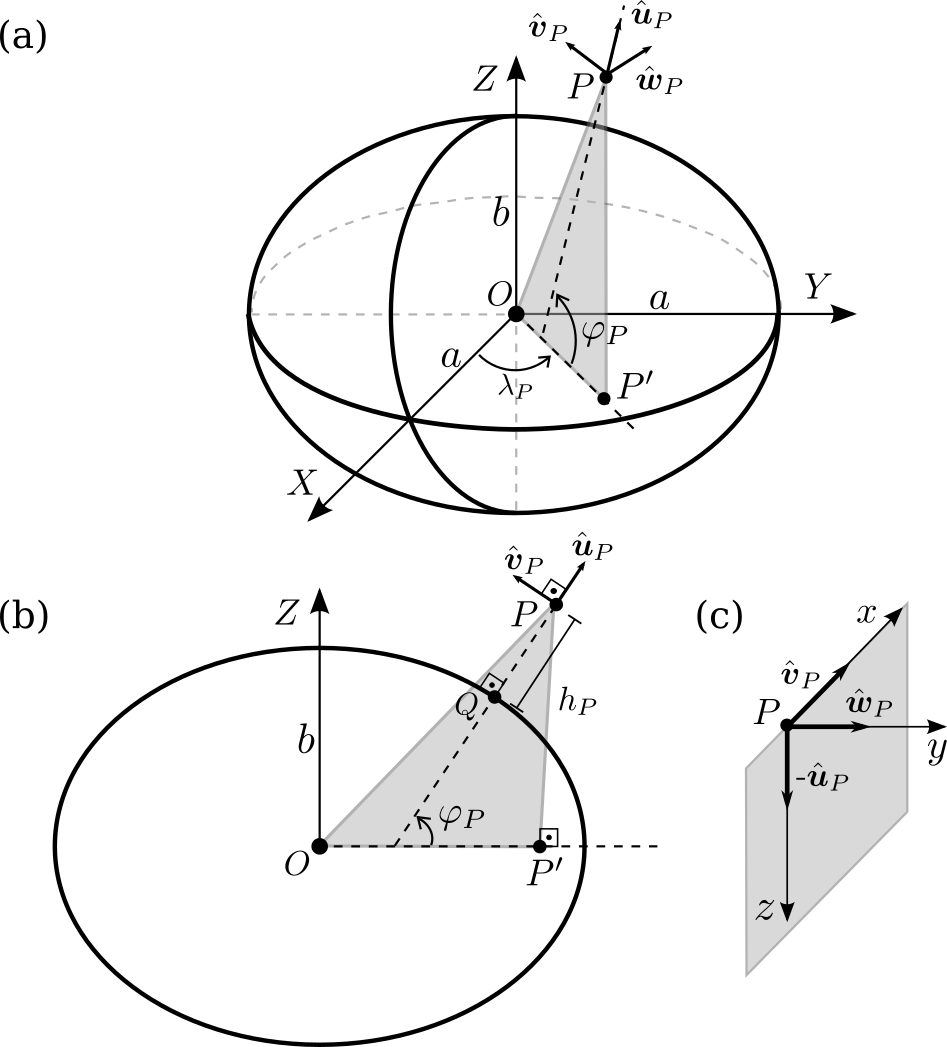
\includegraphics[width=8cm]{figures/cartesian-geodetic-systems.png}%}
    \caption{Schematic representation of the Cartesian and Geodetic systems.}
    \label{fig:cartesian-geodetic-systems}
\end{figure}


\bibliographystyle{gji}

\bibliography{ref}



\appendix
\section{Appendix} \label{appendA}

TEXT TEXT TEXT

\end{document}